\documentclass[UTF8,a4paper]{ctexart}
\usepackage[utf8]{inputenc}
\usepackage{amsmath}
\usepackage{pdfpages}
\usepackage{graphicx}
\usepackage{wrapfig}
\usepackage{listings}
\title{第二次仿真实验报告}
\author{张蔚桐\ 2015011493\ 自55}
\begin {document}
\newcommand{\tabincell}[2]{\begin{tabular}{@{}#1@{}}#2\end{tabular}}
\maketitle
\section{单管BJT放大电路的搭建和仿真测试}
\subsection{静态工作点的调整}
\begin{wrapfigure}{r}{0pt}
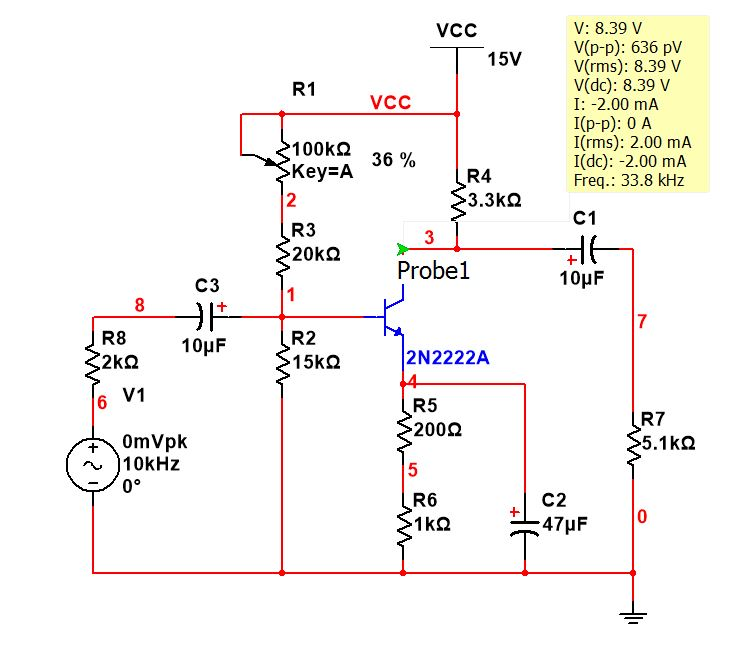
\includegraphics[width=60mm]{1-1.jpg}
\caption{单管BJT放大电路}
\label{bjtc}
\end{wrapfigure}
如图\ref{bjtc}所示是仿真采用的单管放大电路。电路采用阻容耦合方式和射级稳Q电路。经过对变阻器$R_1$的调整,使得如图所示的静态工作电流$I_c=2mA$

下面对$R_1$的数值进行理论计算。经过之前几次的仿真可以知道BJT$\beta\approx220$因此可以得到$I_c\approx I_e\approx 2\rm{mA},U_e=2.4\rm{V}$

进一步,考虑BJT的开启电源$U_{on}\approx0.7\rm{V}$因此可以得到$U_b=3.1\rm{V}$

可以认为三极管基极电流可以忽略不计,那么我们可以得到分压电阻上的电流为
$I=\frac{U_b}{R_2}=0.206\rm{mA}$并进一步得到上拉电阻阻值为$\frac{V_{cc}-U_{b}}{I}=57\mathrm{k}\Omega$

经过仿真测试,可以发现经过调整上拉电阻为$36\mathrm{k}\Omega+20\mathrm{k}\Omega=56\mathrm{k}\Omega$时系统静态工作点满足上述要求,和理论计算基本相符
\subsection{动态参数的测定}
\subsubsection{电压放大倍数的测定}
首先进行理论估算,采用三极管的中频段模型进行估算并设$r_{be}=3\mathrm{k}\Omega$可以迅速得到$A_u=-\frac{\beta(R_c//R_L)}{r_{be}}=-147$

对图\ref{bjtc}的电路外接示波器和失真度仪进行测量,可以得到如图\ref{bjtA}的波形示意图,可以得到电路的仿真放大倍数为$-frac{753+803}{5.24+5.49}=-145$发现和理论计算还是很相近的
\subsubsection{输入电阻的测定}
首先进行理论计算,根据图\ref{bjtc}电路所示,可得输入电阻$R_i=R_2//(R_1+R_3)//r_be\approx2.4\mathrm{k}\Omega$

如图\ref{bjtri}采用半压法对输入电阻进行测量,发现在输入$V_{pp}=10\rm{mV}$即$V_{rms}=7.07\rm{mV}$时,外接电阻$R_8=23.1\mathrm{k}\Omega$时可得到输入分压为3.534mV,因此可得仿真测量输入电阻为$23.1\mathrm{k}\Omega$和理论计算相差不大
\begin{figure}
\centering
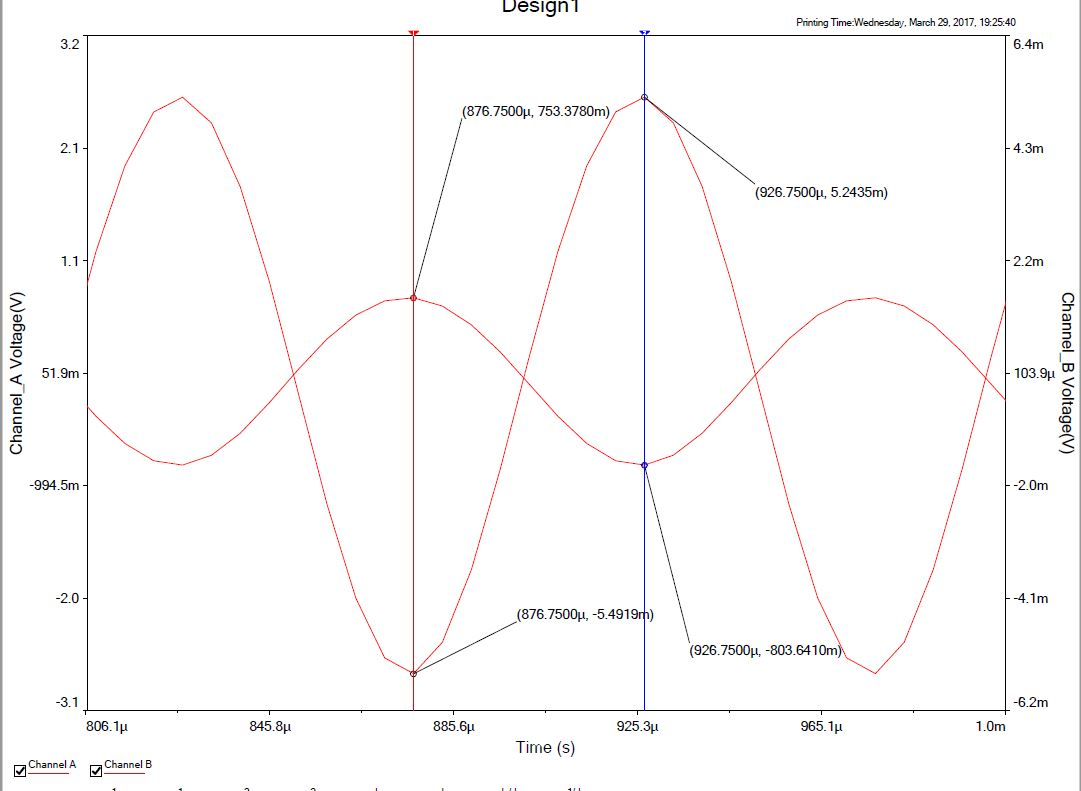
\includegraphics[width=\textwidth]{1-2AA.jpg}
\caption{电压增益的仿真波形曲线}
\label{bjtA}
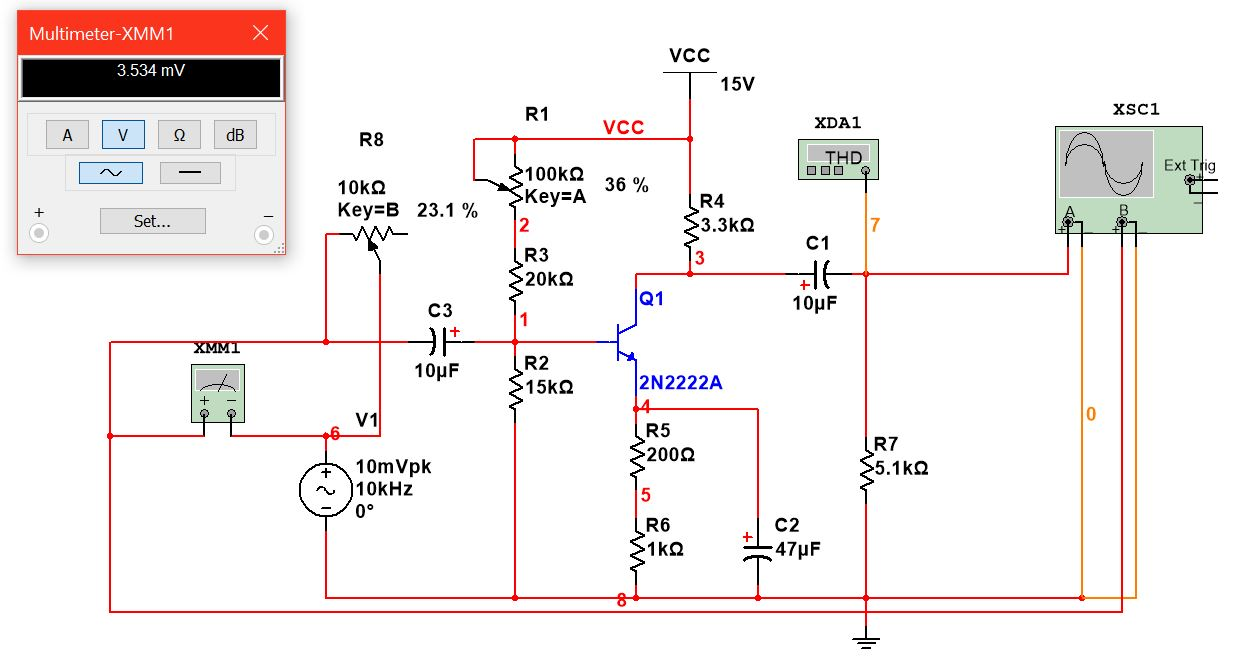
\includegraphics[width=\textwidth]{1-2Ri.jpg}
\caption{放大电路输入电阻的测量}
\label{bjtri}
\end{figure}
\subsection{输出电阻的测量}
理论计算可以迅速得到输出电阻为$3.3\mathrm{k}\Omega$

同样采取半压法进行仿真测试,首先测量空载时的输出电压有效值为888.93mV,如图\ref{bjtuo}所示,外接滑动变阻器如图\ref{bjtro},当调节至3.1$\mathrm{k}\Omega$时发现输出电压为空载输出电压的一半,因此可以得到仿真测试的输出电阻为3.1$mathrm{k}\Omega$和理论计算值相近
\begin{figure}
\centering
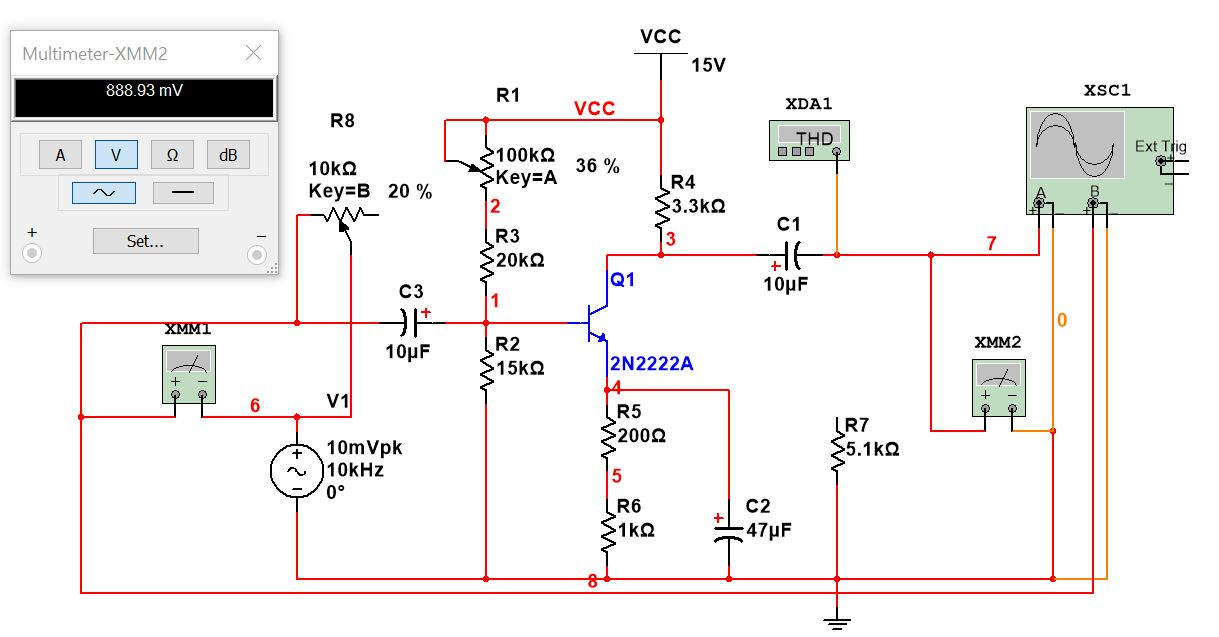
\includegraphics[width=\textwidth]{1-2Uo.jpg}
\caption{放大电路空载输出电压}
\label{bjtuo}
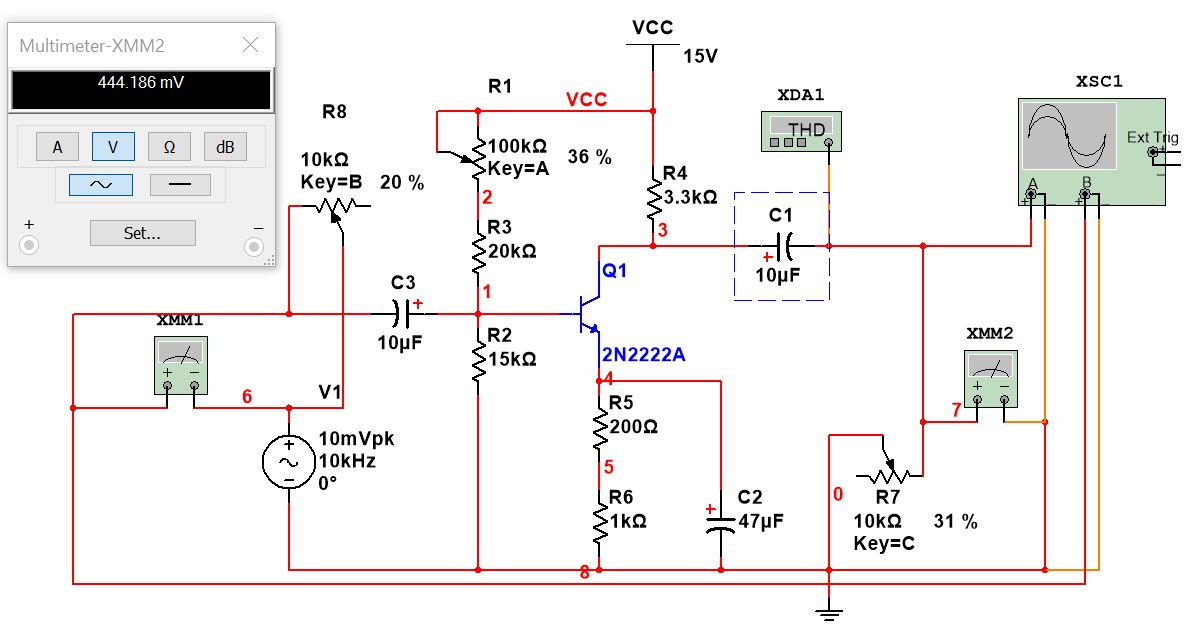
\includegraphics[width=\textwidth]{1-2Ro.jpg}
\caption{放大电路输出电阻的测量}
\label{bjtro}
\end{figure}

\subsubsection{频率响应的测试}
采用$0.707A_{us}$作为上限截止频率和下限截止频率的标准。如图\ref{bjtfl}\ref{bjtfh}所示,可得上限截止频率约为230kHz,下限截止频率为160Hz
\begin{figure}
\centering
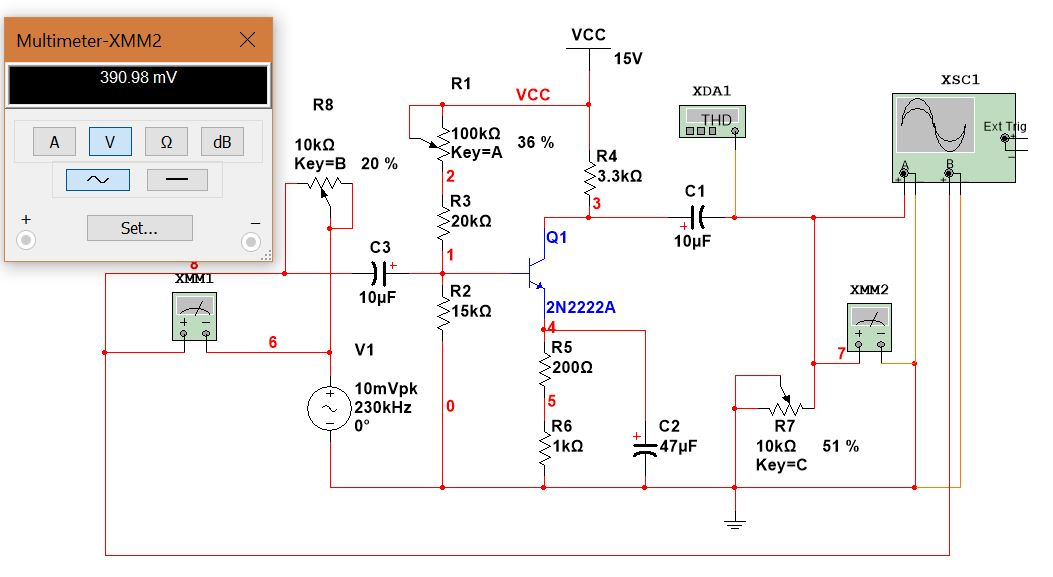
\includegraphics[width=\textwidth]{1-2fh.jpg}
\caption{上限截止频率的测试}
\label{bjtfl}
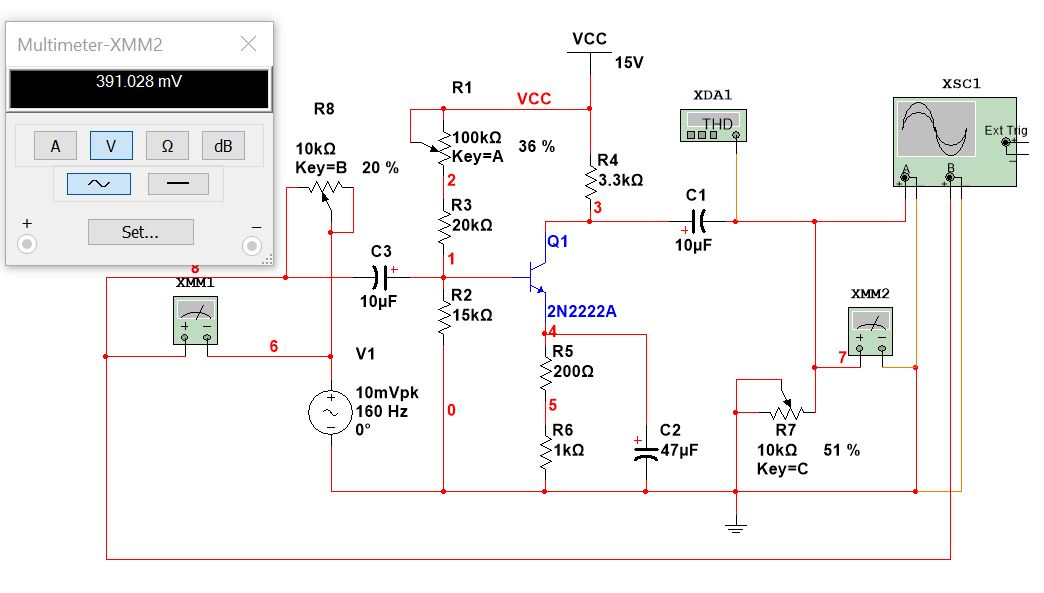
\includegraphics[width=\textwidth]{1-2fl.jpg}
\caption{下限截止频率的测试}
\label{bjtfh}
\end{figure}
\subsection{性能指标的改进}
我们希望在这个电路中能够提供较大的$A_u$,从理论上进行分析可以得到,该电路的$A_u=-\frac{\beta(R_c//R_L)}{r_{be}}$因此为实现目标我们将$R_c$从3.3$\mathrm{k}\Omega$提升至5$\mathrm{k}\Omega$,从理论上进行计算,则可得到$A_u'=-185$得到了上升

如图\ref{bjtc1}对电路进行改进,其中两个滑动变阻器的取值和图\ref{bjtc}中定值电阻的取值是相同的没有影响,可以得到如图\ref{bjtA1}的电压波形曲线,仿真测量的$A_u=-\frac{928+991}{5.16+5.45}=-180$明显得到了提升并和理论估算的值相近。同时,静态工作点没有发生变化

\begin{figure}
\centering
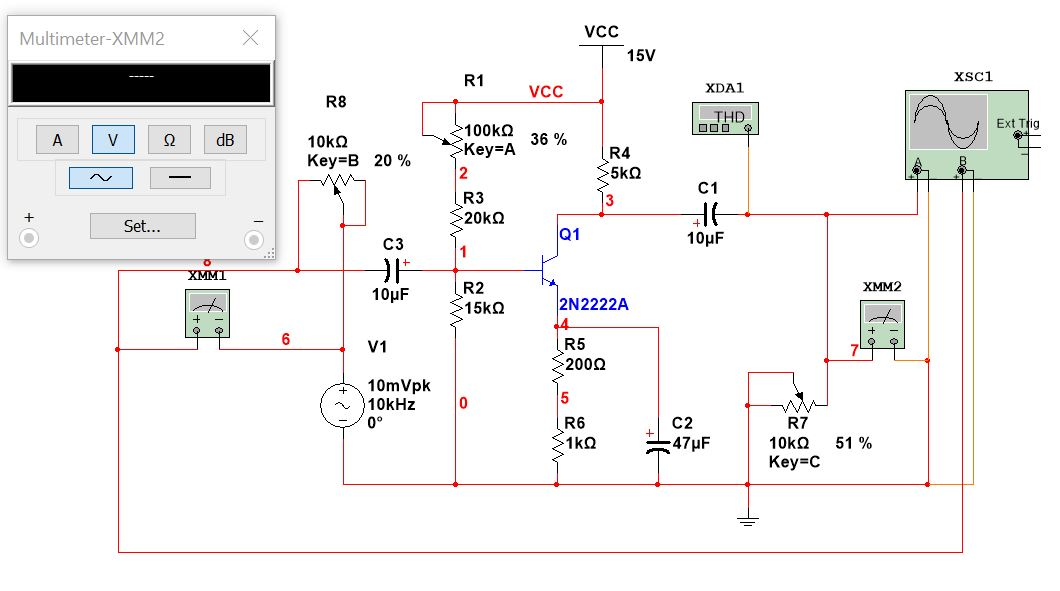
\includegraphics[width=\textwidth]{1-3Ac.jpg}
\caption{对电路的改进}
\label{bjtc1}
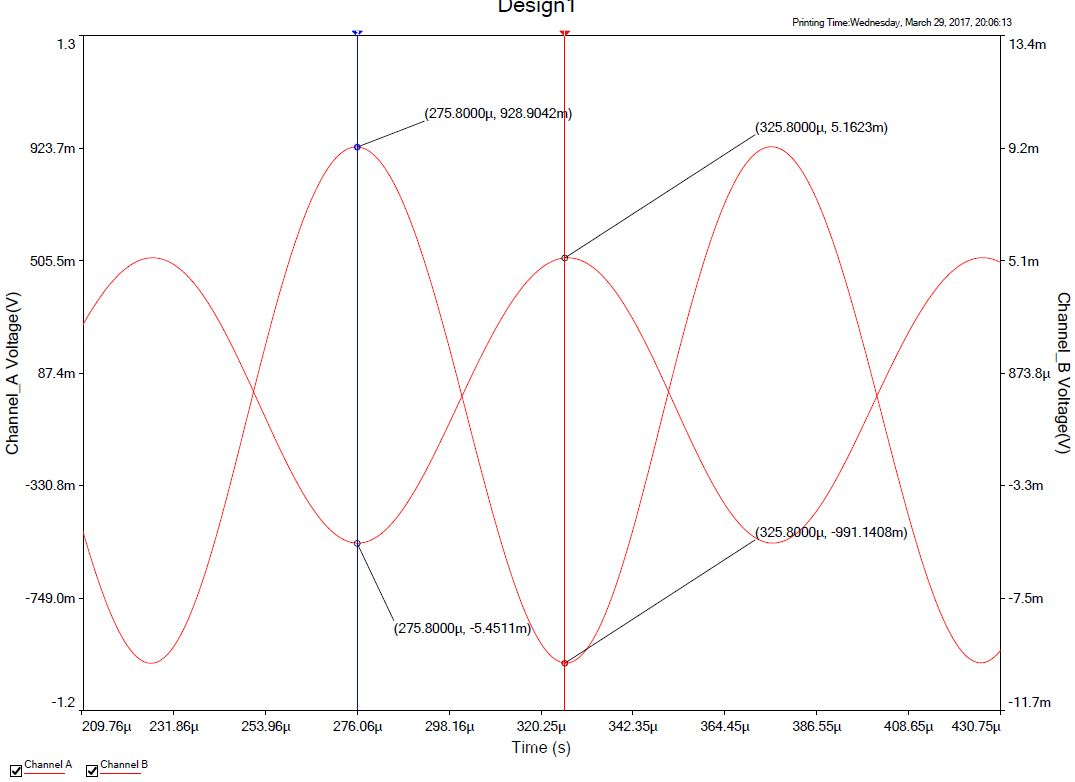
\includegraphics[width=\textwidth]{1-3AA.jpg}
\caption{改进后放大波形}
\label{bjtA1}
\end{figure}
\subsection{失真的产生和消去}

\subsection{实际电路的搭建}
\section{单管MOS放大电路的搭建和仿真测试}
\subsection{datasheet和传输特性的测试}
\subsection{静态工作点的调整}
\subsection{动态参数的测定}
\subsection{性能指标的改进}
\subsection{失真的产生和消去}
\subsection{实际电路的搭建}
\section{集成运放的搭建和仿真测试}
\section{负反馈放大电路自激震荡的产生和消去}
\end{document}